% Don't touch this %%%%%%%%%%%%%%%%%%%%%%%%%%%%%%%%%%%%%%%%%%%
\documentclass[12pt]{article}
\usepackage{fullpage}
\usepackage[left=1in,top=1in,right=1in,bottom=1in,headheight=3ex,headsep=3ex]{geometry}
\usepackage{graphicx}
\usepackage{float}
\usepackage{array}


\newcommand{\blankline}{\quad\pagebreak[2]}
%%%%%%%%%%%%%%%%%%%%%%%%%%%%%%%%%%%%%%%%%%%%%%%%%%%%%%%%%%%%%%

% Modify Course title, instructor name, semester here %%%%%%%%

\title{Practice 2: Steady Flows}
\author{PHY250 - Fall 2021}
\date{}

%%%%%%%%%%%%%%%%%%%%%%%%%%%%%%%%%%%%%%%%%%%%%%%%%%%%%%%%%%%%%%

% Don't touch this %%%%%%%%%%%%%%%%%%%%%%%%%%%%%%%%%%%%%%%%%%%
\usepackage[sc]{mathpazo}
%\linespread{1.05} % Palatino needs more leading (space between lines)
\usepackage[T1]{fontenc}
\usepackage[mmddyyyy]{datetime}% http://ctan.org/pkg/datetime
\usepackage{advdate}% http://ctan.org/pkg/advdate
\newdateformat{syldate}{\twodigit{\THEMONTH}/\twodigit{\THEDAY}}
\newsavebox{\MONDAY}\savebox{\MONDAY}{Mon}% Mon
\newcommand{\week}[1]{%
%  \cleardate{mydate}% Clear date
% \newdate{mydate}{\the\day}{\the\month}{\the\year}% Store date
  \paragraph*{\kern-2ex\quad #1, \syldate{\today} - \AdvanceDate[4]\syldate{\today}:}% Set heading  \quad #1
%  \setbox1=\hbox{\shortdayofweekname{\getdateday{mydate}}{\getdatemonth{mydate}}{\getdateyear{mydate}}}%
  \ifdim\wd1=\wd\MONDAY
    \AdvanceDate[7]
  \else
    \AdvanceDate[7]
  \fi%
}
%\usepackage{setspace}
\usepackage{multicol}
%\usepackage{indentfirst}
\usepackage{fancyhdr,lastpage}
\usepackage{url}
\pagestyle{fancy}
\usepackage{hyperref}
\usepackage{lastpage}
\usepackage{amsmath}
\usepackage{layout}

\lhead{}
\chead{}
%%%%%%%%%%%%%%%%%%%%%%%%%%%%%%%%%%%%%%%%%%%%%%%%%%%%%%%%%%%%%%

% Modify header here %%%%%%%%%%%%%%%%%%%%%%%%%%%%%%%%%%%%%%%%%
%\rhead{\footnotesize Text in header}

%%%%%%%%%%%%%%%%%%%%%%%%%%%%%%%%%%%%%%%%%%%%%%%%%%%%%%%%%%%%%%
% Don't touch this %%%%%%%%%%%%%%%%%%%%%%%%%%%%%%%%%%%%%%%%%%%
\lfoot{}
\cfoot{\small \thepage/\pageref*{LastPage}}
\rfoot{}

\usepackage{array, xcolor}
\usepackage{color,hyperref}
\definecolor{clemsonorange}{HTML}{EA6A20}
\hypersetup{colorlinks,breaklinks,linkcolor=clemsonorange,urlcolor=clemsonorange,anchorcolor=clemsonorange,citecolor=black}

\begin{document}

\maketitle




% First Section %%%%%%%%%%%%%%%%%%%%%%%%%%%%%%%%%%%%%%%%%%%%


\newcounter{example}
\setcounter{example}{1}

\section*{Exercise \theexample}

\textbf{Blood flow}. In humans, blood flows from the heart into the aorta, from which it passes into the major arteries. These branch into the small arteries (arterioles),
 which in turn branch into myriads of tiny capillaries. The blood returns to the heart via the veins. The radius of the aorta is about $1.2 cm$, and the blood passing through it has 
a speed of about $40 cm/s$. A typical capillary has a radius of about $4 \times 10^{-4} cm$, and blood flows through it at a speed of about $5 \times 10^ {-4} m/s$. 


\vspace{5mm}

\begin{figure}[h!]
    \begin{center}
      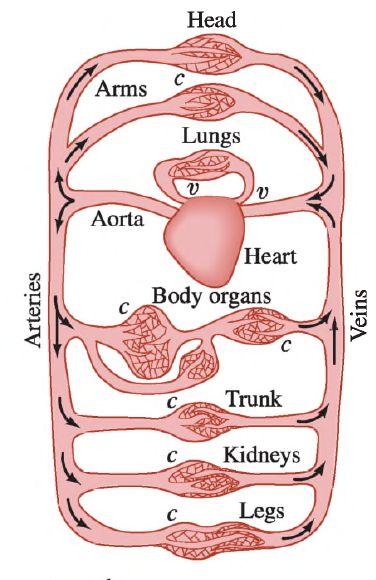
\includegraphics[height=2.5in]{images/hb.jpg}
      \caption{Exercise \theexample }
      \label{1}
    \end{center}
  \end{figure}

% Second Section %%%%%%%%%%%%%%%%%%%%%%%%%%%%%%%%%%%%%%%%%%%%
\stepcounter{example}

\section*{Exercise \theexample}

Calculate the velocity, $v_1$, of a liquid flowing out of a spigot at the bottom of a reservoir.



\vspace{5mm}


\begin{figure}[h!]
  \begin{center}
    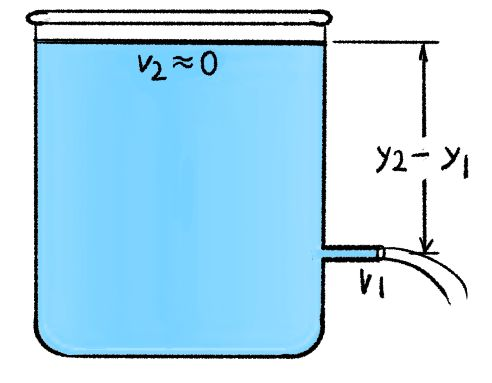
\includegraphics[height=1.3in]{images/Bernoulli2.jpg}
    \caption{Exercise \theexample }
    \label{2}
  \end{center}
\end{figure}

% Third Section %%%%%%%%%%%%%%%%%%%%%%%%%%%%%%%%%%%%%%%%%%%%
\stepcounter{example}

\section*{Exercise \theexample}

The wind speed near the center (“eye”) of a hurricane,
  whose radius is  $30~km$, reaches about $200~km/h$. As air
  swirled in from the rim of the hurricane toward the eye, its angular
  momentum remained roughly constant. (a) Estimate the wind
speed at the rim of the hurricane. (b) Estimate the pressure difference
at the earth’s surface between the eye and the rim.  
Where is the pressure greater? 


% Fourth Section %%%%%%%%%%%%%%%%%%%%%%%%%%%%%%%%%%%%%%%%%%%%
\stepcounter{example}

\section*{Exercise \theexample}


A siphon is a convenient
device for removing liquids from containers. To establish the flow,
the tube must be initially filled with fluid. Let the fluid have density $\rho$
and let the atmospheric pressure be $P_{atm}$. Assume that the
cross-sectional area of the tube is the same at all points along it.
(a) If the lower end of the siphon is at a distance h below the surface
  of the liquid in the container, what is the speed of the fluid as it
  flows out the lower end of the siphon? (Assume that the container
  has a very large diameter, and ignore any effects of viscosity.
(b) A curious feature of a siphon is that the fluid initially flows
  “uphill.” What is the greatest height H that the high point of the
  tube can have if flow is still to occur?


\begin{figure}[h!]
  \begin{center}
    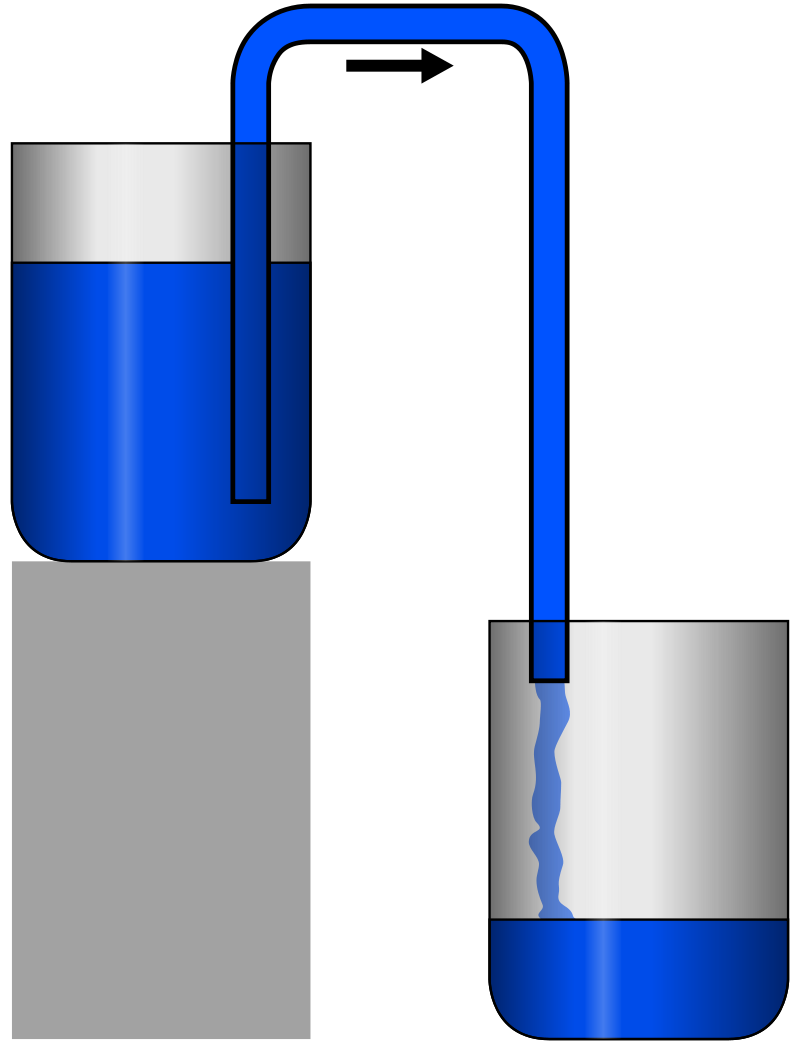
\includegraphics[height=1.8in]{images/Syphon.png}
    \caption{Exercise \theexample }
    \label{3}
  \end{center}
\end{figure}




\end{document}


